\newsavebox{\faceDiagram}
	\sbox{\faceDiagram}	{
		\newcommand{\statcirc}[4]{
	\fill[opacity = 0.5, red,shift={(#1 cm,#2 cm)}, rotate=#3] (0,0) circle (#4); 
	\fill[opacity = 0.5, blue,shift={(#1 cm,#2 cm)},rotate=#3] (0,0) -- (180:#4) arc (180:0:#4) -- cycle;
	%	\draw[->,black,shift={(#1 cm,#2 cm)},rotate=#3] (#4, 0)
}

\newcommand{\drawArrow}[3]{
	\draw[->,>={Stealth[round]}, line width=0.75mm, black ,shift={(#1 cm,#2 cm)}, rotate=#3] (0,-0.5) -- (0,0.5); 
}

\newcommand{\drawchip}[3]{
	\tikzmath
	{
		\chipW = 0.35;
		\chipH = 0.4;
	}
	\fill[opacity = 0.75, darkgray, shift= {(#1 cm, #2 cm)}, rotate = #3, rounded corners] (-\chipH,-\chipW) rectangle (\chipH,\chipW);
	\fill[orange,shift= {(#1 cm, #2 cm)}, rotate = #3 ] (-0.25,0.2) circle (0.1);
}
\begin{tikzpicture}

	\tikzmath{
		\offsetAxis = 0.5;
		\offsetCent = 2.9;
		\diameter = 0.32;
	}
	\draw node (A) at (-0.5, 1.7) {};
	\draw node (B) at (0, 1.7) {};
	\drawchip{\offsetAxis}{\offsetCent}{0};
	\drawchip{-\offsetAxis}{-\offsetCent}{180};
	
	%Magnet North
	\statcirc{-\offsetAxis}{\offsetCent}{70}{\diameter};
	
	\drawArrow{-\offsetAxis}{\offsetCent}{70}
	
	%Magnet EAST
	\statcirc{\offsetCent}{\offsetAxis}{20}{\diameter};
	
	% Magnet West
	\statcirc{\offsetAxis}{-\offsetCent}{190}{\diameter};
	
	\statcirc{-\offsetCent}{-\offsetAxis}{45}{\diameter};
	
	\draw[gray, dashed] (-\offsetAxis,{\offsetCent + 1}) -- 
	(-\offsetAxis,{\offsetCent - 1});
	\draw[black,dotted] (0,0) circle (2.95);
	
	% 4 Cross Lines X
	\draw[black,dashed] (0,0) -- (4,0);
	\draw[black,dashed] (0,0) -- (-4,0);
	\draw[black,dashed] (0,0) -- (0,4);
	\draw[black,dashed] (0,0) -- (0,-4);
	
%	\draw[purple, dotted] ()
	% Dimensioned Variables
	\dimline[line style = {line width = 0.8, arrows = dimline reverse-dimline reverse}] {(A)}{(B)}{x};
	
	% Arc Radius
	\dimline[line style = {line width = 0.8}] {(0,0)} {++(150:2.95)}{R};
%	\dimline {(1,0)}{(-1,0)}{x};
\end{tikzpicture}
	}
	
	\newsavebox{\magnetDigitization}
	\sbox{\magnetDigitization}	{
		
\newcommand{\statcirc}[4]{
	\fill[red,shift={(#1 cm,#2 cm)}, rotate=#3] (0,0) circle (#4); 
	\fill[blue,shift={(#1 cm,#2 cm)},rotate=#3] (0,0) -- (180:#4) arc (180:0:#4) -- cycle;
	%	\draw[->,black,shift={(#1 cm,#2 cm)},rotate=#3] (#4, 0)
}

\newcommand{\drawArrow}[3]{
	\draw[->,>={Stealth[round]}, line width=0.75mm, black ,shift={(#1 cm,#2 cm)}, rotate=#3] (0,-1) -- (0,1); 
}

\begin{tikzpicture}[scale = 0.75]
\tikzmath{
	\offsetAxis = 0.5;
	\offsetCent = 2.9;
	\diameter = 0.75;
}

\foreach \i in {1,...,30}
{
	\draw[gray] (0,0) -- (\i * 12-6 : 2.8);
	\node[inner sep=0pt] at (-{\i * 12}+12: 3) {\i};
}
\node[circle,draw,inner sep=0pt, fill = green] at (-{18 * 12}+12: 3) {18};
\statcirc{0}{0}{-204-90}{\diameter};
\drawArrow{0}{0}{-204-90};
\draw[black,dashed] (0,0) -- (3,0);
\draw[black,dashed] (0,0) -- (-3,0);
\draw[black,dashed] (0,0) -- (0,3);
\draw[black,dashed] (0,0) -- (0,-3);
\draw[gray, dotted] (0,0) -- (-204: 3);
\draw[gray, dotted] (0,0) -- (-204: 3);
\draw [white, line width = 5pt] (2.1,0)  arc (0:360-204:2.1);
\draw [<->, >={Stealth[round]}] (2.1,0)  arc (0:360-204:2.1);
\node[circle,inner sep=3pt, fill = white]				at (90:2) {$\theta$};
\end{tikzpicture}
	}
	
	\newsavebox{\gridFigure}
	\sbox{\gridFigure}	{
		\begin{tikzpicture}[every node/.style={minimum size=2 cm-\pgflinewidth, outer sep=0pt}]
    \draw[step=2cm,color=black] (0,0) grid (4,4);

    \node[fill=orange] at (+1,+1) {};
   % \node[fill=yellow] at (+0.75,+0.75) {};
\end{tikzpicture}
	}
	%\begin{tikzpicture}[minimum width = 14 cm, minimum height = 6 cm]
	%\draw (0,0) -- (14,6);
	
	\begin{tikzpicture}[]
	%complexnode/.pic={\usebox{\mybox}}]
	
	\newcommand\xa{2};
	\newcommand\xb{2};
	\newcommand\ya{2};
	\newcommand\yb{2};
	
	\coordinate (smallNE) at (2,5);
	\coordinate (smallSE) at (2,5);
	\coordinate (smallSW) at (2,5);
	\coordinate (smallNW) at (2,5);
	
	\coordinate (bigNE) at (2,5);
	\coordinate (bigSE) at (2,5);
	\coordinate (bigSW) at (2,5);
	\coordinate (bigSE) at (2,5);
	
	\node[opacity = 0.95] at (3.15 cm, 2.85 cm) {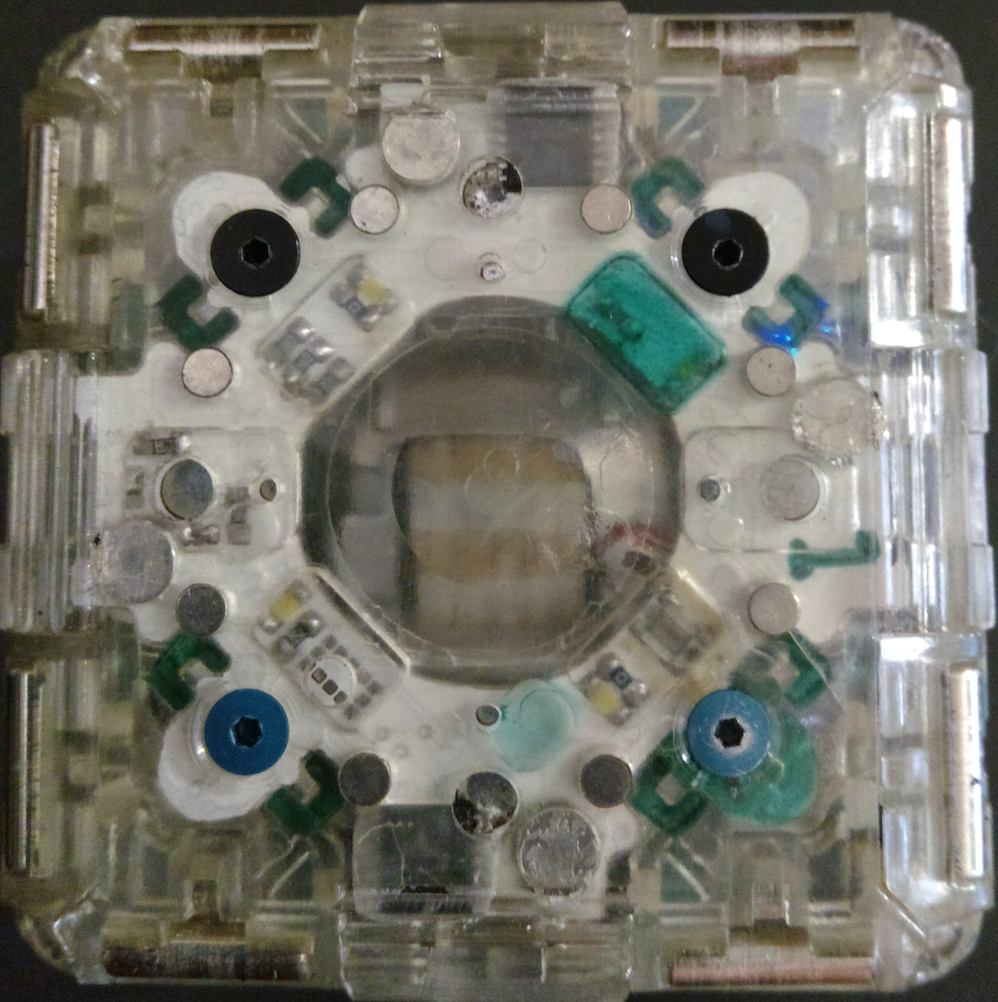
\includegraphics[width = 5.9 cm]{figures/face.png}};
	\node at (3 cm, 3 cm) {\usebox{\faceDiagram}};
	\node at (10 cm, 3 cm) {\usebox{\magnetDigitization}};
	\node at (15.5 cm, 2cm) {\usebox{\gridFigure}};
	
	%\node[fill=orange] at (3,3) {\textbf{18}};
	
	\tikzmath{
		\smallBoxX = 0.5;
		\smallBoxY = 2.9;
	}

	% Small Box around Magnet
	%\node[draw, purple, dotted, minimum size = 1.25 cm, rounded corners, thick] at (3.65cm , 7cm) {};
	
	\path[draw, purple, dotted, minimum size = 1.25 cm, rounded corners, ultra thick]
	(3*0.7, 6.25*0.7) --
	++(1.25, 0) --
	++(0, 1.25) --
	++(-1.25, 0) --
	cycle {};
	
	\node (a) at (12.5, 3){};
	\node (b) at (14.75, 3.4){};
	
	\draw[>={Stealth[round]}, purple,dashed, ultra thick, bend right, rounded corners = 1 cm, ->] (a) -- (13.75,5) -- (b);
	
	\draw[purple,dashed, thin] (2.7cm, 4.35cm + 1.25cm) -- ++(358: 4.8cm);
	\draw[purple,dashed, thin] (2.7cm, 4.35cm ) -- ++(323: 5.9cm);
	
	% Large Purple box
	\node[draw, purple, dotted, minimum size = 5 cm, rounded corners,ultra thick] at (10cm , 3cm) {};
	
	\node[] at (10cm , 0.2cm) {Discretizing Angle};
	%\draw (1,1) pic {complexnode} (4,4);
	
	\end{tikzpicture}
	
	
	
	
%	\newsavebox{\faceDiagram}
%	\sbox{\faceDiagram}	{
%		\newcommand{\statcirc}[4]{
	\fill[opacity = 0.5, red,shift={(#1 cm,#2 cm)}, rotate=#3] (0,0) circle (#4); 
	\fill[opacity = 0.5, blue,shift={(#1 cm,#2 cm)},rotate=#3] (0,0) -- (180:#4) arc (180:0:#4) -- cycle;
	%	\draw[->,black,shift={(#1 cm,#2 cm)},rotate=#3] (#4, 0)
}

\newcommand{\drawArrow}[3]{
	\draw[->,>={Stealth[round]}, line width=0.75mm, black ,shift={(#1 cm,#2 cm)}, rotate=#3] (0,-0.5) -- (0,0.5); 
}

\newcommand{\drawchip}[3]{
	\tikzmath
	{
		\chipW = 0.35;
		\chipH = 0.4;
	}
	\fill[opacity = 0.75, darkgray, shift= {(#1 cm, #2 cm)}, rotate = #3, rounded corners] (-\chipH,-\chipW) rectangle (\chipH,\chipW);
	\fill[orange,shift= {(#1 cm, #2 cm)}, rotate = #3 ] (-0.25,0.2) circle (0.1);
}
\begin{tikzpicture}

	\tikzmath{
		\offsetAxis = 0.5;
		\offsetCent = 2.9;
		\diameter = 0.32;
	}
	\draw node (A) at (-0.5, 1.7) {};
	\draw node (B) at (0, 1.7) {};
	\drawchip{\offsetAxis}{\offsetCent}{0};
	\drawchip{-\offsetAxis}{-\offsetCent}{180};
	
	%Magnet North
	\statcirc{-\offsetAxis}{\offsetCent}{70}{\diameter};
	
	\drawArrow{-\offsetAxis}{\offsetCent}{70}
	
	%Magnet EAST
	\statcirc{\offsetCent}{\offsetAxis}{20}{\diameter};
	
	% Magnet West
	\statcirc{\offsetAxis}{-\offsetCent}{190}{\diameter};
	
	\statcirc{-\offsetCent}{-\offsetAxis}{45}{\diameter};
	
	\draw[gray, dashed] (-\offsetAxis,{\offsetCent + 1}) -- 
	(-\offsetAxis,{\offsetCent - 1});
	\draw[black,dotted] (0,0) circle (2.95);
	
	% 4 Cross Lines X
	\draw[black,dashed] (0,0) -- (4,0);
	\draw[black,dashed] (0,0) -- (-4,0);
	\draw[black,dashed] (0,0) -- (0,4);
	\draw[black,dashed] (0,0) -- (0,-4);
	
%	\draw[purple, dotted] ()
	% Dimensioned Variables
	\dimline[line style = {line width = 0.8, arrows = dimline reverse-dimline reverse}] {(A)}{(B)}{x};
	
	% Arc Radius
	\dimline[line style = {line width = 0.8}] {(0,0)} {++(150:2.95)}{R};
%	\dimline {(1,0)}{(-1,0)}{x};
\end{tikzpicture}
%	}
%	
%	\newsavebox{\magnetDigitization}
%	\sbox{\magnetDigitization}	{
%		
\newcommand{\statcirc}[4]{
	\fill[red,shift={(#1 cm,#2 cm)}, rotate=#3] (0,0) circle (#4); 
	\fill[blue,shift={(#1 cm,#2 cm)},rotate=#3] (0,0) -- (180:#4) arc (180:0:#4) -- cycle;
	%	\draw[->,black,shift={(#1 cm,#2 cm)},rotate=#3] (#4, 0)
}

\newcommand{\drawArrow}[3]{
	\draw[->,>={Stealth[round]}, line width=0.75mm, black ,shift={(#1 cm,#2 cm)}, rotate=#3] (0,-1) -- (0,1); 
}

\begin{tikzpicture}[scale = 0.75]
\tikzmath{
	\offsetAxis = 0.5;
	\offsetCent = 2.9;
	\diameter = 0.75;
}

\foreach \i in {1,...,30}
{
	\draw[gray] (0,0) -- (\i * 12-6 : 2.8);
	\node[inner sep=0pt] at (-{\i * 12}+12: 3) {\i};
}
\node[circle,draw,inner sep=0pt, fill = green] at (-{18 * 12}+12: 3) {18};
\statcirc{0}{0}{-204-90}{\diameter};
\drawArrow{0}{0}{-204-90};
\draw[black,dashed] (0,0) -- (3,0);
\draw[black,dashed] (0,0) -- (-3,0);
\draw[black,dashed] (0,0) -- (0,3);
\draw[black,dashed] (0,0) -- (0,-3);
\draw[gray, dotted] (0,0) -- (-204: 3);
\draw[gray, dotted] (0,0) -- (-204: 3);
\draw [white, line width = 5pt] (2.1,0)  arc (0:360-204:2.1);
\draw [<->, >={Stealth[round]}] (2.1,0)  arc (0:360-204:2.1);
\node[circle,inner sep=3pt, fill = white]				at (90:2) {$\theta$};
\end{tikzpicture}
%	}
%	
%	\newsavebox{\gridFigure}
%	\sbox{\gridFigure}	{
%		\begin{tikzpicture}[every node/.style={minimum size=2 cm-\pgflinewidth, outer sep=0pt}]
    \draw[step=2cm,color=black] (0,0) grid (4,4);

    \node[fill=orange] at (+1,+1) {};
   % \node[fill=yellow] at (+0.75,+0.75) {};
\end{tikzpicture}
%	}
%	%\begin{tikzpicture}[minimum width = 14 cm, minimum height = 6 cm]
%	%\draw (0,0) -- (14,6);
%	
%	\begin{tikzpicture}[]
%	%complexnode/.pic={\usebox{\mybox}}]
%	
%	\newcommand\xa{2};
%	\newcommand\xb{2};
%	\newcommand\ya{2};
%	\newcommand\yb{2};
%	
%	\coordinate (smallNE) at (2,5);
%	\coordinate (smallSE) at (2,5);
%	\coordinate (smallSW) at (2,5);
%	\coordinate (smallNW) at (2,5);
%	
%	\coordinate (bigNE) at (2,5);
%	\coordinate (bigSE) at (2,5);
%	\coordinate (bigSW) at (2,5);
%	\coordinate (bigSE) at (2,5);
%	
%	\node[opacity = 0.95] at (4.25 cm, 4 cm) {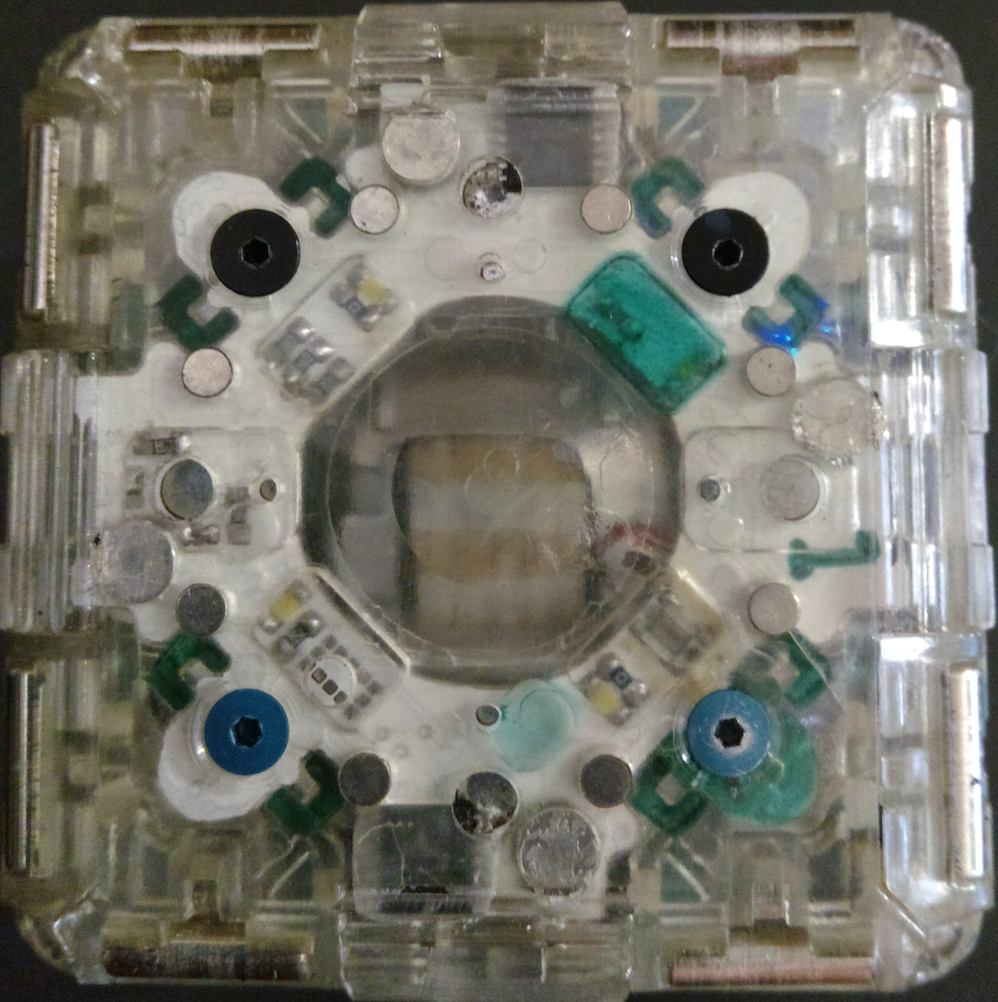
\includegraphics[width = 8 cm]{figures/face.png}};
%	\node at (4 cm, 4 cm) {\usebox{\faceDiagram}};
%	\node at (11 cm, 6 cm) {\usebox{\magnetDigitization}};
%	\node at (15 cm, 2cm) {\usebox{\gridFigure}};
%	
%	%\node[fill=orange] at (3,3) {\textbf{18}};
%	
%	\tikzmath{
%		\smallBoxX = 0.5;
%		\smallBoxY = 2.9;
%	}
%	
%	% Small Box around Magnet
%	%\node[draw, purple, dotted, minimum size = 1.25 cm, rounded corners, thick] at (3.65cm , 7cm) {};
%	
%	\path[draw, purple, dotted, minimum size = 1.25 cm, rounded corners, ultra thick]
%	(3, 6.25) --
%	++(1.25, 0) --
%	++(0, 1.25) --
%	++(-1.25, 0) --
%	cycle {};
%	
%	\node (a) at (13.5, 6){};
%	\node (b) at (15.75, 3.5){};
%	\draw[>={Stealth[round]}, purple,dashed, ultra thick, bend right, rounded corners = 1 cm, ->] (a) -- (15.75,6) -- (b);
%	\draw[purple,dashed, thin] (3.5cm, 6.25cm + 1.25cm) -- ++(10: 5cm);
%	\draw[purple,dashed, thin] (3.5cm, 6.25cm ) -- ++(332: 5.45cm);
%	
%	% Large Purple box
%	\node[draw, purple, dotted, minimum size = 4.8 cm, rounded corners,ultra thick] at (11cm , 6cm) {};
%	
%	%\draw (1,1) pic {complexnode} (4,4);
%	
%	\end{tikzpicture}